% Section content template for individual Educative lessons
% This file contains the actual content for a specific section
% Generated from Educative API section content

% Section: Requirements of Quora's Design
% Section ID: 6254998790340608
% Section Slug: requirements-of-quoras-design
% Generated: 2025-12-07T22:55:24.646325

\subsection{Requirements}\label{pf-ig1Ag6_Dx3YeAi0cfq}
\\
Let's understand the functional and non-functional requirements below:\\

\subsubsection{Functional requirements}\label{0gybILG6eeWRVpIQLXtMn}
\\
A user should be able to perform the following functionalities:

\begin{itemize}
\item
\protect\phantomsection\label{g69vNOuK69x6aF30E1pYx}
\textbf{Questions and answers}: Users can ask questions and give answers. Questions and answers can include images and videos.
\item
\protect\phantomsection\label{NHDycTTbdMpciU7GoG5xi}
\textbf{Upvote/downvote and comment}: It is possible for users to upvote, downvote, and comment on answers.
\item
\protect\phantomsection\label{5D9gFDpOkp6QT2uWba01S}
\textbf{Search}: Users should have a search feature to find questions already asked on the platform by other users.
\item
\protect\phantomsection\label{tCEYFaHDI2VPEkAXt3NOz}
\textbf{Recommendation system}: A user can view their feed, which includes topics they're interested in. The feed can also include questions that need answers or answers that interest the reader. The system should facilitate user discovery with a recommender system.
\item
\protect\phantomsection\label{Wgk4bHIKS432dLflJ1rFm}
\textbf{Ranking answers}: We enhance user experience by ranking answers according to their usefulness. The most helpful answer will be ranked highest and listed at the top.
\end{itemize}

\subsubsection{Non-functional requirements}\label{Rb3KOMsaTasqO-VhM2r2R}

\begin{itemize}
\item
\protect\phantomsection\label{ggByKT6JXNZApiVbLAcUn}
\textbf{Scalability}: The system should scale well as the number of features and users grow with time. It means that the performance and usability should not be impacted by an increasing number of users.
\item
\protect\phantomsection\label{L1u85vAD2ZlmC2mu2_vri}
\textbf{Consistency}: The design should ensure that different users' views of the same content should be consistent. In particular, critical content like questions and answers should be the same for any collection of viewers. However, it is not necessary that all users of Quora see a newly posted question, answer, or comment right away.
\item
\protect\phantomsection\label{ydEM4lnx07YgfmBKXc92i}
\textbf{Availability}: The system should have high availability. This applies to cases where servers receive a large number of concurrent requests.
\item
\protect\phantomsection\label{W-sJuNFEoaFp8b9Qydsvy}
\textbf{Performance}: The system should provide a smooth experience to the user without a noticeable delay.
\end{itemize}

\begin{figure}[htbp]
 \centering
 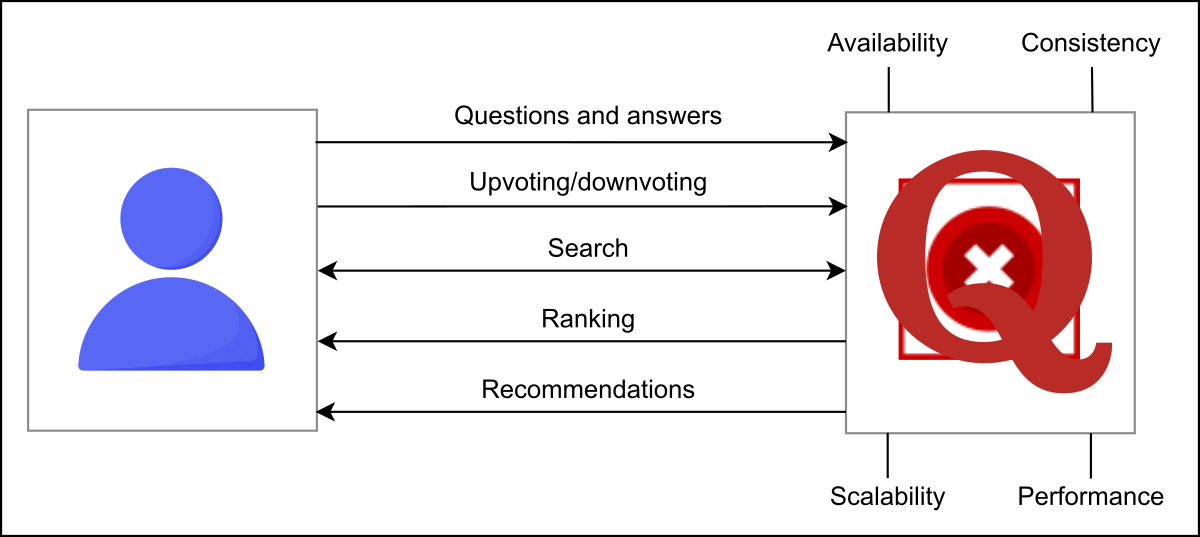
\includegraphics[width=0.5\textwidth]{Images/chapter_27/section_6254998790340608/4760235149754368.png}
 \caption{Functional and non-functional requirements of Quora}
\end{figure}

\subsection{Resource estimation}\label{0VFUGUyEh5B3VSF_uX52P}
\\
In this section, we'll make an estimate about the resource requirements for Quora service. We 'll make assumptions to get a practical and tractable estimate. We
'll estimate the number of servers, the storage, and the bandwidth required to facilitate a large number of users.
\\
\textbf{Assumptions}: It is important to base our estimation on some underlying assumptions. We, therefore, assume the following:

\begin{itemize}
\item
\protect\phantomsection\label{SpHmwrOziJ8FdHw5XD_oT}
There are a total of 1 billion users, out of which 300 million are daily active users.
\item
\protect\phantomsection\label{D0zzGBu9GJ5xVRPrEouUR}
Assume 15\% of questions have an image, and 5\% of questions have a video embedded in them. A question cannot have both at the same time.
\item
\protect\phantomsection\label{yk9lfYj6zCsV774qmau_c}
We'll assume an image is estimated to be 250 KBs, and a video is considered 5 MBs.
\end{itemize}

\subsubsection{Number of servers estimation}\label{8x9pjB_sIFhlIArddfIVO}
\\
Since we have 300 million daily active users for Quora. Considering
\href{https://www.educative.io/courses/grokking-the-system-design-interview/put-back-of-the-envelope-numbers-in-perspective}{our assumption} of using daily active users as a proxy for the number of requests per second to find the number of servers for peak load times, we get 300 million requests per second. Then
, we use the following formula to calculate the number of servers:

\[
\text{Servers needed at peak load} = \frac{\text{Number of requests/second}}{\text{RPS of server}}
\]

Using \href{https://www.educative.io/courses/grokking-the-system-design-interview/put-back-of-the-envelope-numbers-in-perspective}{64,000 as an estimated RPS a server can handle}, the required servers are estimated as follows:

\[
\text{Servers needed at peak load = } \frac{300\ \text{million}}{64,000} = 4687.5 \approx 4.7\text{K servers}
\]

\begin{figure}[htbp]
 \centering
 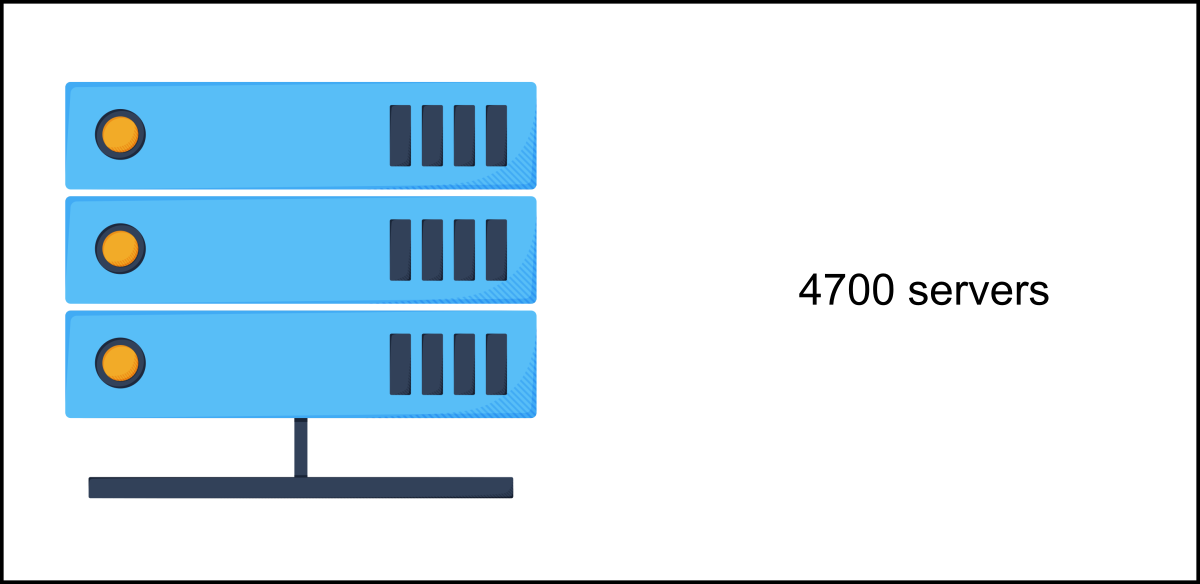
\includegraphics[width=0.5\textwidth]{Images/chapter_27/section_6254998790340608/5825528487870464.png}
 \caption{The estimated number of servers required for Quora}
\end{figure}

\subsubsection{Storage estimation}\label{KBPVzXQT8QBvoLNr47Zkr}
\\
Let's keep in mind our assumption that 15\% of questions have images and 5\% have videos. So , we'll make the following assumptions to estimate the storage requirements for our design:

\begin{itemize}
\item
\protect\phantomsection\label{yna9wmVFkOGFw1ARVss_f}
Each of the 300 million active users posts 1 question in a day, and each question has 2 responses on average, 10 upvotes, and 5 comments in total.
\item
\protect\phantomsection\label{nTl_S2VsbimX6wh1cbE2b}
The collective storage required for the textual content (including the question, answer(s), and comment(s) text) of one question equals \protect\phantomsection\label{katex_inline_VLg_1x0jvl5HIob7P6gzt}{{{\(100\ \text{KB}\)}}}.
\end{itemize}

The following are the default calculations:

\begin{itemize}
\tightlist
\item
Total questions: \(300M \times 1 = 300 \times 10^6\) questions per day.
\item
Storage required for textual content of all questions in one day: \(300 \times M \times 1 \times 100
\times {10^3} B= 30TB\)
\item
Storage required for images for one day: \(\frac{300 \times 10^6 \times 15}{100} \times 250 \times 10^3 B= 11.25TB\)
\item
Storage required for video content for one day: \(\frac{300 \times 10^6 \times 5}{100} \times 5 \times 10^6 B= 75TB\)
\end{itemize}

\begin{figure}[htbp]
 \centering
 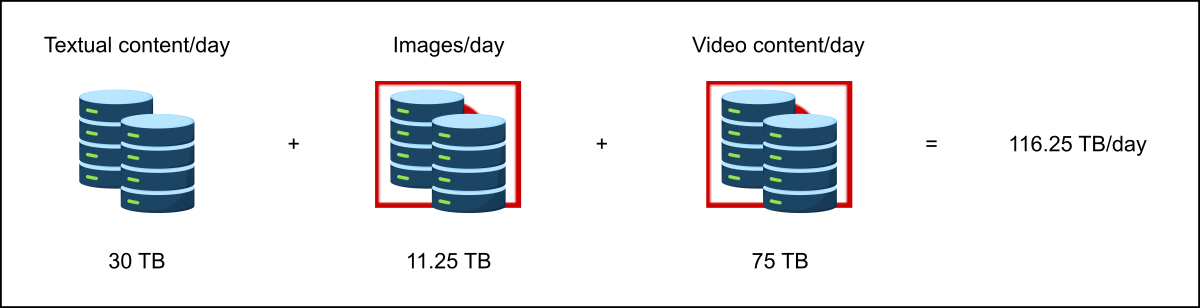
\includegraphics[width=0.5\textwidth]{Images/chapter_27/section_6254998790340608/5794914866954240.png}
 \caption{Summarizing storage requirements of Quora}
\end{figure}

\begin{quote}
\protect\phantomsection\label{katex_inline_ifKG8ePCXMBd7nNSIf4-I}{{{\(\text{Total storage required for one day} = 30\ \text{TB} + 11.25\ \text{TB} + 75\ \text{TB} \approx 116.25\ \text{TB/day}\)}}}
\end{quote}
\\
The daily storage requirements of Quora seem very high. But for service with 300 million DAU, a yearly requirement of \protect\phantomsection\label{katex_inline_-xZwDbjKRHo9hi6lmE3cr}{{{\(116.25\ \text{TB} \times 365 = 42.43\ \text{PB}\)}}} is feasible. The practical requirement will be much higher because we have disregarded the storage required for a number of things. For example, non-active (out of \protect\phantomsection\label{katex_inline_wDapInxzK15EGm1wPws2X}{{{\(1\text{ B}\)}}}) users\textquotesingle{} data will require storage.

\subsubsection{Bandwidth estimation}\label{trufkZpBjN9d1lxm4Q1-V}
\\
The bandwidth estimate requires the calculation of incoming and outgoing data through the network.

\begin{itemize}
\item
\protect\phantomsection\label{F3euJbHky1zBrESuThh-M}
\textbf{Incoming traffic}: The incoming traffic bandwidth required per day will be equal to \protect\phantomsection\label{katex_inline_yy52X1sP4SicgWQQUB1yU}{{{\(\frac{116.25\ \text{TB}}{86,400} \times 8 = 10.9\ \text{Gbps} \approx 11\ \text{Gbps}\)}}}
\item
\protect\phantomsection\label{VPpJWjtCTo5fueUA1X4o9}
\textbf{Outgoing traffic}: We have assumed that 300 million active users views 20 questions per day, so the total bandwidth requirements can be found in the calculator below:
\end{itemize}

\begin{itemize}
\tightlist
\item
\(300 M \times 20\ questions = 6\) billion questions are viewed per day.
\item
Questions viewed per second: \(\frac{6 \times 10^9}{86400} ~= 69.4 \times 10^3\) questions are viewed per second.
\item
Bandwidth for the textual content of all questions and their answers: \(69.4 \times 10^3 \times 100 \times 10^3 \times 8\ bits = 55.56\ Gbps\)
\item
Bandwidth of the 15\% of content which contain images per second: \(69.4 \times 10^3 \times \frac{15}{100} \times 250 \times 10^3 \times 8\ bits = 20.83\ Gbps\)
\item
Bandwidth for the 5\% of content that contains video per second: \(69.4 \times 10^3 \times \frac{5}{100} \times 5 \times 10^6 \times 8\ bits = 138.9\ Gbps\)
\item
Total outgoing traffic bandwidth: \(55.56\ Gbps + 20.82\ Gbps + 138.9\ Gbps = 215.3\ Gbps\)
\end{itemize}
\\
We use rounding at each step in this explanation. The answers in the calculator above are slightly different due to rounding.

\begin{figure}[htbp]
 \centering
 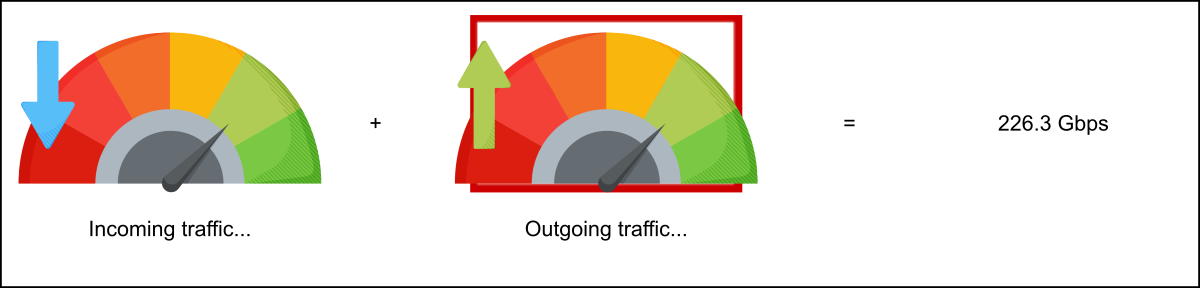
\includegraphics[width=0.5\textwidth]{Images/chapter_27/section_6254998790340608/5003887386165248.png}
 \caption{Summarizing the bandwidth requirements of Quora}
\end{figure}

\hfill\break
Total bandwidth requirement of Quora is equal to:
\begin{quote}
Incoming + outgoing traffic bandwidth \protect\phantomsection\label{katex_inline_qdPb9IsgEBM8uC1k9sAaI}{{{\(\text{= 11 Gbps + 215.3 Gbps = 226.3 Gbps}\)}}}
\end{quote}
\subsection{Building blocks we will use}\label{354Aj_bIFPzMcuOYOkHxB-1}
\\
We'll use the following building blocks for the initial design of Quora:

\begin{figure}[htbp]
 \centering
 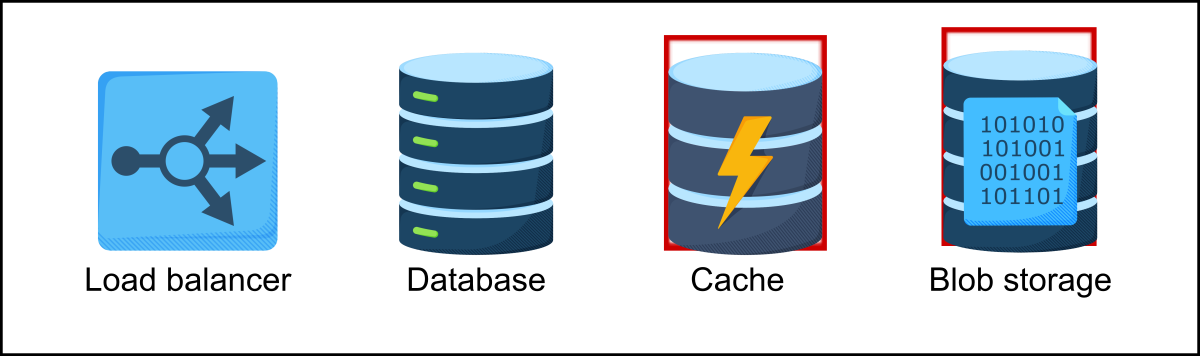
\includegraphics[width=0.5\textwidth]{Images/chapter_27/section_6254998790340608/6200125401989120.png}
 \caption{Building blocks required for our design}
\end{figure}

\begin{itemize}
\item
\protect\phantomsection\label{r8Dyv_TvmK3xToc8Dumme}
\href{https://www.educative.io/courses/grokking-the-system-design-interview/introduction-to-load-balancers}{\textbf{Load balancers}} will be used to divide the traffic load among the service hosts.
\item
\protect\phantomsection\label{oogB1R_A0cUz8Nk2p5xud}
\href{https://www.educative.io/courses/grokking-the-system-design-interview/introduction-to-databases}{\textbf{Databases}} are essential for storing all sorts of data, such as user questions and answers, comments, and likes and dislikes. Also, user data will be stored in the databases. We may use different types of databases to store different data.
\item
\protect\phantomsection\label{R5cKyBKOq3m1AUGdPUOsy}
\href{https://www.educative.io/courses/grokking-the-system-design-interview/system-design-the-distributed-cache}{\textbf{A distributed caching system}} will be used to store frequently accessed data. We can also use caching to store our view counters for different questions.
\item
\protect\phantomsection\label{AVqdMn2t0g4S46XTg-_BT}
\href{https://www.educative.io/courses/grokking-the-system-design-interview/system-design-a-blob-store}{\textbf{The blob store}} will keep images and video files.
\end{itemize}

% End of section content